\section{Experimental results}\label{sec:results}

To give comparative results on the quality of the initialisation processes
considered in this work, four well-known, categorical, labelled datasets ---
breast cancer, mushroom, nursery, and soybean (large) --- will be clustered by
the \(k\)-modes algorithm with each of the initialisation processes. These
datasets have been chosen to fall in line with the established literature, and
for their relative sizes and complexities. Each dataset is openly available
under the UCI Machine Learning Repository~\cite{Dua2019}, and their
characteristics are summarised in Table~\ref{tab:dataset_summary}.

\begin{table}[htbp]
    \resizebox{\textwidth}{!}{%
        \begin{tabular}{lrrrlrr}
\toprule
{} &  No. rows &  No. cols &  No. classes &  Missing values &  Adjusted no. rows &  Adjusted no. classes \\
\midrule
Breast cancer &       699 &        10 &            2 &            True &                683 &                     2 \\
Mushroom      &      8124 &        22 &            2 &            True &               5644 &                     2 \\
Soybean       &       307 &        35 &           19 &            True &                266 &                    15 \\
Nursery       &     12960 &         8 &            5 &           False &              12960 &                     5 \\
\bottomrule
\end{tabular}

    }\caption{A summary of the benchmark datasets.}\label{tab:dataset_summary}
\end{table}

Clustering algorithms are often evaluated based on their performance as a
classifier~\cite{%
    Arthur2007,Cao2009,Cao2012,Huang1998,Ng2007,Olaode2014,Schaeffer2007%
}. This is a fundamentally flawed approach --- especially given that
classification belongs to an entirely different branch of learning. Moreover,
doing so requires a number of assumptions about the topology of the data within
the metric space that is being considered~\cite{Memoli2011}. One such assumption
is that the classes recorded in the data are indeed separable objects like
clusters.

This analysis does not consider evaluative metrics related to classification
such as accuracy, recall or precision. Instead, only internal measures are
considered such as the cost function defined in~\eqref{eq:cost}. This metric is
label-invariant and its values are comparable across the different
initialisation methods. Furthermore, the effect of each initialisation method
on the initial and final clusterings can be captured with the cost function. An
additional, and often useful, metric is the silhouette coefficient. This
measures the ratio between the intra-cluster cohesion and inter-cluster
separation of a particular clustering. Therefore, it could be used in a similar
way to reveal the effect of each initialisation method at the beginning and end
of a run of \(k\)-modes. Unfortunately, this metric loses its intuition under
the distance measure employed here and is omitted. The remaining performance
measures used are the number of iterations for the \(k\)-modes algorithm to
terminate and the time taken to terminate in seconds.

The final piece of information required in this analysis is a choice for \(k\)
for each dataset. An immediate choice is the number of classes that are present
in a dataset but, as stated above, this is not necessarily a fair or wise choice
since the classes may not be representative of true clusters. A popular strategy
for choosing an optimal number of clusters is known as the `elbow' method. The
aim of this method is to identify a kink (elbow) in a plot of number of clusters
against cost for a dataset. This kink suggests that an increase in \(k\) from
there would not sufficiently improve the performance of the model. On its own,
this method is vague and somewhat unreliable which raises a number of questions:
\begin{itemize}
    \item What constitutes a kink?
    \item How does one discern between multiple kinks?
    \item Is the decision subjective with respect to the observer?
\end{itemize}

Alas, an alternative `elbow' may be identified objectively by using
the knee point detection algorithm~\cite{Satopaa2011} where the maximal
value of \(k\) is taken to be \(\lfloor\sqrt{N}\rfloor\). This algorithm
identifies the value of \(k\) with the maximum curvature in the plot described
above by computation rather than inspection --- eliminating the concerns raised.
An example plot for the nursery dataset is given in
Figure~\ref{fig:nursery_costs} where the clustering is performed using Cao's
method.

\begin{figure}
    \centering
    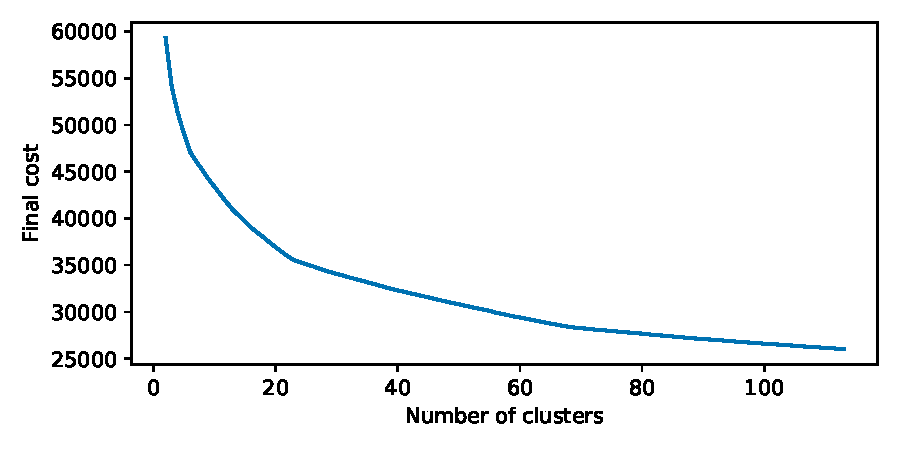
\includegraphics[width=.6\linewidth]{./img/elbow/nursery_costs.pdf}
    \caption{An elbow plot for the nursery dataset using Cao's initialisation
             method.}\label{fig:nursery_costs}
\end{figure}

\subsection{Elbow method}
\graphicspath{{./img/elbow/}}

Tables~\ref{tab:breast_cancer_summary_elbow}---\ref{tab:soybean_summary_elbow}
summarise the results of each initialisation method on the benchmark datasets
where the number of clusters has been determined by the knee point detection
algorithm. Each column shows the mean value of each metric and its standard
deviation in parentheses over 250
independent
repetitions of the \(k\)-modes algorithm.

\begin{table}
    \centering
    \resizebox{\textwidth}{!}{%
        \begin{tabular}{lllll}
\toprule
{} &      Initial cost &        Final cost & No. iterations &          Time \\
\midrule
Cao      &   2178.00 (0.000) &   1955.00 (0.000) &   4.00 (0.000) &  0.37 (0.025) \\
Huang    &  2123.12 (92.805) &  2023.80 (49.390) &   2.58 (0.810) &  0.25 (0.054) \\
Matching &  2110.68 (87.670) &  2015.42 (40.354) &   2.72 (0.834) &  0.21 (0.034) \\
\bottomrule
\end{tabular}

    }
    \captionof{table}{Summative metric results for the breast cancer dataset
    with \(k=8\).}\label{tab:breast_cancer_summary_elbow}\vspace{20pt}

    \resizebox{\textwidth}{!}{%
        \begin{tabular}{lllll}
\toprule
{} &         Initial cost &           Final cost & No. iterations &          Time \\
\midrule
Cao      &     29922.00 (0.000) &     29621.00 (0.000) &   2.00 (0.000) &  1.78 (0.066) \\
Huang    &  35112.67 (3286.612) &  31312.27 (1387.005) &   2.98 (1.012) &  2.74 (0.758) \\
Matching &  35237.67 (3201.877) &  31183.28 (1143.908) &   2.99 (0.924) &  1.79 (0.421) \\
\bottomrule
\end{tabular}

    }
    \captionof{table}{Summative metric results for the mushroom dataset with
    \(k=17\).}\label{tab:mushroom_summary_elbow}\vspace{20pt}

    \resizebox{\textwidth}{!}{%
        \begin{tabular}{lllll}
\toprule
{} &        Initial cost &          Final cost & No. iterations &          Time \\
\midrule
Cao      &    35544.00 (0.000) &    35544.00 (0.000) &   1.00 (0.000) &  4.98 (0.152) \\
Huang    &  37535.06 (372.596) &  37535.06 (372.596) &   1.00 (0.000) &  3.58 (0.121) \\
Matching &  37484.29 (327.467) &  37484.29 (327.467) &   1.00 (0.000) &  3.14 (0.141) \\
\bottomrule
\end{tabular}

    }
    \captionof{table}{Summative metric results for the nursery dataset with
    \(k=23\).}\label{tab:nursery_summary_elbow}\vspace{20pt}

    \resizebox{\textwidth}{!}{%
        \begin{tabular}{lllll}
\toprule
{} &       Initial cost &        Final cost & No. iterations &          Time \\
\midrule
Cao      &    1822.00 (0.000) &   1700.00 (0.000) &   4.00 (0.000) &  0.24 (0.009) \\
Huang    &  1964.56 (107.504) &  1832.92 (61.820) &   3.36 (0.875) &  0.23 (0.043) \\
Matching &   1929.50 (85.928) &  1829.54 (68.632) &   3.44 (1.110) &  0.15 (0.027) \\
\bottomrule
\end{tabular}

    }
    \captionof{table}{Summative metric results for the soybean dataset with
    \(k=8\).}\label{tab:soybean_summary_elbow}
\end{table}

\begin{figure}
    \begin{minipage}{.5\textwidth}
        \includegraphics[width=\linewidth]%
            {breast_cancer_cost_scatterplot.pdf}
    \end{minipage}
    \begin{minipage}{.5\textwidth}
        \includegraphics[width=\linewidth]%
            {breast_cancer_initial_cost_cdfplot.pdf}

        \includegraphics[width=\linewidth]%
            {breast_cancer_final_cost_cdfplot.pdf}
    \end{minipage}
\end{figure}

\begin{figure}
    \begin{minipage}{.5\textwidth}
        \includegraphics[width=\linewidth]%
            {mushroom_cost_scatterplot.pdf}
    \end{minipage}
    \begin{minipage}{.5\textwidth}
        \includegraphics[width=\linewidth]%
            {mushroom_initial_cost_cdfplot.pdf}

        \includegraphics[width=\linewidth]%
            {mushroom_final_cost_cdfplot.pdf}
    \end{minipage}
\end{figure}

\begin{figure}
    \begin{minipage}{.5\textwidth}
        \includegraphics[width=\linewidth]%
            {soybean_cost_scatterplot.pdf}
    \end{minipage}
    \begin{minipage}{.5\textwidth}
        \includegraphics[width=\linewidth]%
            {soybean_initial_cost_cdfplot.pdf}

        \includegraphics[width=\linewidth]%
            {soybean_final_cost_cdfplot.pdf}
    \end{minipage}
\end{figure}

\begin{figure}
    \begin{minipage}{.5\textwidth}
        \includegraphics[width=\linewidth]%
            {nursery_cost_scatterplot.pdf}
    \end{minipage}
    \begin{minipage}{.5\textwidth}
        \includegraphics[width=\linewidth]%
            {nursery_initial_cost_cdfplot.pdf}

        \includegraphics[width=\linewidth]%
            {nursery_final_cost_cdfplot.pdf}
    \end{minipage}
\end{figure}


\subsection{Number of classes}
\graphicspath{{./img/nclasses/}}

\begin{table}
    \centering
    \resizebox{\textwidth}{!}{%
        \begin{tabular}{lllll}
\toprule
{} &       Initial cost &         Final cost & No. iterations &          Time \\
\midrule
Cao      &    3315.00 (0.000) &    3172.00 (0.000) &   2.00 (0.000) &  0.13 (0.005) \\
Huang    &  3393.80 (120.772) &  3348.51 (144.849) &   1.54 (0.653) &  0.10 (0.024) \\
Matching &  3406.73 (111.686) &  3355.56 (144.621) &   1.61 (0.638) &  0.09 (0.018) \\
\bottomrule
\end{tabular}

    }
    \captionof{table}{Summative metric results for the breast cancer dataset
    with \(k=8\).}\label{tab:breast_cancer_summary_nclasses}\vspace{20pt}

    \resizebox{\textwidth}{!}{%
        \begin{tabular}{lllll}
\toprule
{} &         Initial cost &           Final cost & No. iterations &          Time \\
\midrule
Cao      &     37662.00 (0.000) &     37662.00 (0.000) &   1.00 (0.000) &  1.10 (0.142) \\
Huang    &  41720.20 (2519.647) &  38612.64 (2086.246) &   3.14 (1.471) &  2.04 (0.759) \\
Matching &  42297.98 (2265.532) &  39496.56 (2681.581) &   3.36 (1.439) &  1.62 (0.567) \\
\bottomrule
\end{tabular}

    }
    \captionof{table}{Summative metric results for the mushroom dataset with
    \(k=17\).}\label{tab:mushroom_summary_nclasses}\vspace{20pt}

    \resizebox{\textwidth}{!}{%
        \begin{tabular}{lllll}
\toprule
{} &        Initial cost &          Final cost & No. iterations &          Time \\
\midrule
Cao      &    35544.00 (0.000) &    35544.00 (0.000) &   1.00 (0.000) &  4.98 (0.152) \\
Huang    &  37535.06 (372.596) &  37535.06 (372.596) &   1.00 (0.000) &  3.58 (0.121) \\
Matching &  37484.29 (327.467) &  37484.29 (327.467) &   1.00 (0.000) &  3.14 (0.141) \\
\bottomrule
\end{tabular}

    }
    \captionof{table}{Summative metric results for the nursery dataset with
    \(k=23\).}\label{tab:nursery_summary_nclasses}\vspace{20pt}

    \resizebox{\textwidth}{!}{%
        \begin{tabular}{lllll}
\toprule
{} &       Initial cost &        Final cost & No. iterations &          Time \\
\midrule
Cao      &    1822.00 (0.000) &   1700.00 (0.000) &   4.00 (0.000) &  0.24 (0.009) \\
Huang    &  1964.56 (107.504) &  1832.92 (61.820) &   3.36 (0.875) &  0.23 (0.043) \\
Matching &   1929.50 (85.928) &  1829.54 (68.632) &   3.44 (1.110) &  0.15 (0.027) \\
\bottomrule
\end{tabular}

    }
    \captionof{table}{Summative metric results for the soybean dataset with
    \(k=8\).}\label{tab:soybean_summary_nclasses}
\end{table}

\begin{figure}
    \begin{minipage}{.5\textwidth}
        \includegraphics[width=\linewidth]%
            {breast_cancer_cost_scatterplot.pdf}
    \end{minipage}
    \begin{minipage}{.5\textwidth}
        \includegraphics[width=\linewidth]%
            {breast_cancer_initial_cost_cdfplot.pdf}

        \includegraphics[width=\linewidth]%
            {breast_cancer_final_cost_cdfplot.pdf}
    \end{minipage}
\end{figure}

\begin{figure}
    \begin{minipage}{.5\textwidth}
        \includegraphics[width=\linewidth]%
            {mushroom_cost_scatterplot.pdf}
    \end{minipage}
    \begin{minipage}{.5\textwidth}
        \includegraphics[width=\linewidth]%
            {mushroom_initial_cost_cdfplot.pdf}

        \includegraphics[width=\linewidth]%
            {mushroom_final_cost_cdfplot.pdf}
    \end{minipage}
\end{figure}

\begin{figure}
    \begin{minipage}{.5\textwidth}
        \includegraphics[width=\linewidth]%
            {soybean_cost_scatterplot.pdf}
    \end{minipage}
    \begin{minipage}{.5\textwidth}
        \includegraphics[width=\linewidth]%
            {soybean_initial_cost_cdfplot.pdf}

        \includegraphics[width=\linewidth]%
            {soybean_final_cost_cdfplot.pdf}
    \end{minipage}
\end{figure}

\begin{figure}
    \begin{minipage}{.5\textwidth}
        \includegraphics[width=\linewidth]%
            {nursery_cost_scatterplot.pdf}
    \end{minipage}
    \begin{minipage}{.5\textwidth}
        \includegraphics[width=\linewidth]%
            {nursery_initial_cost_cdfplot.pdf}

        \includegraphics[width=\linewidth]%
            {nursery_final_cost_cdfplot.pdf}
    \end{minipage}
\end{figure}

